\documentclass[11pt,letterpaper]{report}

\usepackage[margin=1in]{geometry}
\usepackage{titlesec}
\usepackage{fancyhdr}
\usepackage{graphicx}
\usepackage{longtable}
\usepackage{array}
\usepackage{booktabs}
\usepackage{xcolor}
\usepackage{listings}
\usepackage{enumitem}
\usepackage{hyperref}
\usepackage{parskip}
\usepackage{caption}
\usepackage{seqsplit}

\graphicspath{{../../screenshots/}}

\definecolor{codebg}{HTML}{F5F5F5}
\definecolor{codeframe}{HTML}{CCCCCC}
\definecolor{accent}{HTML}{2454FF}

\lstset{
  basicstyle=\ttfamily\small,
  backgroundcolor=\color{codebg},
  frame=single,
  rulecolor=\color{codeframe},
  breaklines=true,
  breakatwhitespace=false,
  columns=fullflexible,
  showstringspaces=false,
  tabsize=2,
  captionpos=b,
  xleftmargin=1em,
  xrightmargin=1em,
}

\hypersetup{
  colorlinks=true,
  linkcolor=accent,
  urlcolor=accent,
  citecolor=accent,
  pdftitle={EventPass -- Requirements, Design \& Implementation Report},
  pdfauthor={EventPass Project},
}

\setlength{\headheight}{14pt}
\pagestyle{fancy}
\fancyhf{}
\fancyhead[L]{EventPass}
\fancyhead[R]{\leftmark}
\fancyfoot[C]{\thepage}
\renewcommand{\headrulewidth}{0.4pt}

\titleformat{\chapter}[hang]{\Huge\bfseries}{\thechapter.}{1em}{}
\titlespacing*{\chapter}{0pt}{0pt}{2em}

\newcommand{\code}[1]{\lstinline[breaklines=true]{#1}}

\begin{document}

% ---------------------------------------------------------------- Title page
\begin{titlepage}
  \centering
  \vspace*{3cm}
  {\Huge\bfseries EventPass\par}
  \vspace{0.5cm}
  {\Large Event Ticketing \& Check-in System\par}
  \vspace{1.5cm}
  {\large Requirements, Design \& Implementation Report\par}
  \vspace{2cm}
  {\large CSCD602 -- Advanced Software Engineering\par}
  {\large Capstone -- 48-Hour Individual Exam Project\par}
  \vfill
  {\large \today\par}
\end{titlepage}

\tableofcontents

% ==================================================================
\chapter{Overview}
% ==================================================================

EventPass is a small event ticketing and check-in tool built for a
single organizer role: create events, register attendees against them,
and check attendees in at the door using a system-generated ticket
code -- typed by hand, or scanned as a QR code.

The system is a conventional two-tier web application:

\begin{itemize}[leftmargin=1.5em]
  \item \textbf{Backend} -- Node.js, Express, and SQLite (via
    \code{better-sqlite3}), exposing a JSON REST API under \code{/api}.
  \item \textbf{Frontend} -- React (Vite), a single-page app that
    consumes that API.
\end{itemize}

It was scoped and built under a time-boxed exam constraint, which
shaped several deliberate choices documented throughout this report:
SQLite over a client-server database to avoid setup friction, a single
organizer role rather than a full permissions model, and one
non-functional requirement -- correct check-in behavior under
concurrent requests -- treated as the one property worth an automated,
adversarial test rather than manual spot-checking.

This report is organized in three parts: requirements and scope
(Chapter~\ref{ch:requirements}), the data model and API design
(Chapter~\ref{ch:design}), and the implementation itself
(Chapter~\ref{ch:implementation}), followed by how the system was
verified (Chapter~\ref{ch:testing}) and what was deliberately left out
(Chapter~\ref{ch:scope}).

% ==================================================================
\chapter{Requirements \& Scope}
\label{ch:requirements}
% ==================================================================

This chapter is reverse-documented from the shipped implementation --
it describes what the system actually does and enforces, not an
aspirational spec written before the code existed.

\section{Actors}

\begin{description}[leftmargin=2em]
  \item[Organizer] The only authenticated role. Registers an account,
    creates events, registers attendees, and checks people in. Can
    only see and modify their own events and attendees.
  \item[Attendee] Never logs in. Exists only as a row created by an
    organizer, identified by a ticket code. Presents that code (or its
    QR encoding) at the door.
\end{description}

There is no admin role, no multi-organizer collaboration on one event,
and no self-service attendee registration -- an organizer enters every
attendee by hand.

\section{Functional Requirements}

Numbered to match how they map onto the API and the automated test
suite, not an external spec -- kept here for traceability between this
document, the API design in Chapter~\ref{ch:design}, and the tests in
Chapter~\ref{ch:testing}.

\begin{description}[leftmargin=3.2em, style=nextline]
  \item[FR1] An organizer can register an account with name, email,
    and password. Email must be unique across all organizers.
  \item[FR2] An organizer can log in with email/password and receive a
    bearer token valid for 12 hours.
  \item[FR3] An organizer can create an event with a name and date
    (required), plus optional venue and capacity.
  \item[FR4] An organizer can list, view, update, and delete only
    their own events.
  \item[FR5] Deleting an event deletes its attendees too -- no
    orphaned attendee rows.
  \item[FR6] An organizer can register an attendee (name + email) to
    one of their own events.
  \item[FR7] The same email cannot be registered twice for the
    \emph{same} event, but can be registered for different events.
  \item[FR8] Every registered attendee is issued a ticket code,
    generated by the system -- the organizer does not supply it. The
    code is guaranteed unique across all attendees, not just within
    one event.
  \item[FR9] An organizer can look up a ticket by code without
    checking it in (e.g.\ to verify it before someone reaches the
    door).
  \item[FR10] An organizer/staff member can check in a ticket by code.
    A successful check-in records a timestamp.
  \item[FR11] A ticket can only be checked in once. A second attempt
    on an already-checked-in code is rejected -- not silently
    accepted, not double-recorded -- and reports when the first
    check-in happened.
  \item[FR12] Checking in a code that doesn't exist is rejected and is
    distinguishable from ``already checked in'' (different HTTP status
    code).
  \item[FR13] An event's detail view shows live counts: how many are
    registered, how many are checked in, and the check-in percentage.
  \item[FR14] A ticket's code is also rendered as a scannable QR code
    (encoding the raw code string) so it can be checked in without
    manual typing, and can be printed per attendee.
\end{description}

\section{Non-Functional Requirements}

\begin{description}[leftmargin=3.6em, style=nextline]
  \item[NFR1 -- Check-in correctness under concurrency] The critical
    failure mode for a system like this is double-admitting one ticket
    because two devices scanned it in the same instant. FR11 must
    hold even when multiple check-in requests for the same code
    arrive concurrently -- exactly one succeeds, the rest are rejected
    as duplicates. This is the one requirement with a dedicated
    automated test firing simultaneous requests
    (Section~\ref{sec:concurrency-test}), because it is the one
    requirement that is easy to get wrong with a naive
    read-then-write implementation and hard to catch by manual
    testing.
  \item[NFR2 -- Data isolation] One organizer must never be able to
    read or modify another organizer's events, attendees, or tickets,
    even with a valid token for their own account. Enforced by
    scoping every query to \code{organizerId = req.user.id} (directly
    for events, via the owning event for attendees/tickets).
  \item[NFR3 -- Zero-install local setup] SQLite via
    \code{better-sqlite3} needs no external database service, so
    \code{npm install \&\& npm run dev} in both \code{backend/} and
    \code{frontend/} is the entire setup -- chosen because setup
    friction is wasted time under a time-boxed exam constraint.
  \item[NFR4 -- Fast, keyboard/scanner-friendly check-in] The
    \code{/checkin} screen auto-focuses its input and refocuses after
    every submission, so a staff member scanning a QR code (which
    types-and-submits like a keyboard) or typing codes by hand can
    process a queue without touching the mouse between attendees.
  \item[NFR5 -- Ticket codes must be legible when read aloud or
    transcribed by hand] Seven characters, uppercase letters and
    digits, with \code{0}/\code{O} and \code{1}/\code{I} excluded from
    the alphabet.
\end{description}

\section{Acceptance Criteria (as tested)}
\label{sec:acceptance}

The backend test suite is the executable version of the acceptance
criteria considered important enough to automate:

\begin{enumerate}[leftmargin=1.8em]
  \item Generated ticket codes match the expected shape (7 characters,
    excluded-ambiguous-character alphabet), and
    \code{generateUniqueTicketCode} never returns a code already
    present in the database, across repeated generation against a
    growing table.
  \item A valid, unused ticket code checks in successfully and
    returns a timestamp (FR10).
  \item Checking in the same code twice returns \code{409} on the
    second call, with the \emph{original} check-in time, not a new
    one (FR11).
  \item Checking in an unknown code returns \code{404} (FR12).
  \item Five simultaneous check-in requests against one fresh code
    result in exactly 1 success and 4 conflicts (NFR1).
  \item Registering the same email twice to the same event is
    rejected with \code{409 DUPLICATE_EMAIL} (FR7).
\end{enumerate}

Everything else (auth, event CRUD, stats, the QR/print UI) was
verified by manual and scripted browser-driven testing rather than an
automated suite -- see Chapter~\ref{ch:testing}.

% ==================================================================
\chapter{Data Model \& API Design}
\label{ch:design}
% ==================================================================

\section{Entity-Relationship Overview}

Three tables carry the whole system: \code{users}, \code{events}, and
\code{attendees}. A ``ticket'' is not a separate row -- it is the
\code{ticketCode}/\code{checkedIn}/\code{checkedInAt} columns on an
\code{attendees} row.

\begin{center}
\begin{tabular}{p{2.6cm}p{5.5cm}p{5.5cm}}
\toprule
\textbf{Table} & \textbf{Relationship} & \textbf{Role} \\
\midrule
\code{users} & referenced by \code{events.organizerId} & one organizer account \\
\code{events} & belongs to a \code{users} row; parent of \code{attendees} & one event owned by one organizer \\
\code{attendees} & belongs to an \code{events} row & one registered attendee / ticket \\
\bottomrule
\end{tabular}
\end{center}

\section{Schema}

\subsection{\code{users}}
\begin{center}
\begin{tabular}{p{3cm}p{2cm}p{8cm}}
\toprule
\textbf{Column} & \textbf{Type} & \textbf{Notes} \\
\midrule
\code{id} & TEXT & UUID v4, primary key \\
\code{name} & TEXT & required \\
\code{email} & TEXT & required, unique \\
\code{passwordHash} & TEXT & bcrypt, 10 rounds \\
\code{createdAt} & TEXT & defaults to \code{datetime('now')} \\
\bottomrule
\end{tabular}
\end{center}

\subsection{\code{events}}
\begin{center}
\begin{tabular}{p{3cm}p{2cm}p{8cm}}
\toprule
\textbf{Column} & \textbf{Type} & \textbf{Notes} \\
\midrule
\code{id} & TEXT & UUID v4, primary key \\
\code{organizerId} & TEXT & FK $\rightarrow$ \code{users.id} \\
\code{name} & TEXT & required \\
\code{date} & TEXT & required, free-form (frontend sends \code{datetime-local}) \\
\code{venue} & TEXT & optional \\
\code{capacity} & INTEGER & optional, \emph{not enforced anywhere} (see Chapter~\ref{ch:scope}) \\
\code{createdAt} & TEXT & defaults to \code{datetime('now')} \\
\bottomrule
\end{tabular}
\end{center}

\subsection{\code{attendees}}
\begin{center}
\begin{tabular}{p{3cm}p{2cm}p{8cm}}
\toprule
\textbf{Column} & \textbf{Type} & \textbf{Notes} \\
\midrule
\code{id} & TEXT & UUID v4, primary key \\
\code{eventId} & TEXT & FK $\rightarrow$ \code{events.id} \\
\code{name} & TEXT & required \\
\code{email} & TEXT & required \\
\code{ticketCode} & TEXT & unique across the whole table, 7 characters \\
\code{checkedIn} & INTEGER & 0/1, default 0 \\
\code{checkedInAt} & TEXT & null until checked in \\
\code{createdAt} & TEXT & defaults to \code{datetime('now')} \\
\bottomrule
\end{tabular}
\end{center}

Constraints: \code{UNIQUE(ticketCode)} and \code{UNIQUE(eventId, email)}
-- the same email can register for two different events, but not
twice for the same one. Indexes exist on \code{ticketCode} and
\code{eventId} on \code{attendees}, and on \code{organizerId} on
\code{events} -- the three columns everything is looked up by.

\subsection{Ticket codes}

Generated in \code{backend/src/utils/ticketCode.js}: 7 characters from
the alphabet \texttt{\seqsplit{ABCDEFGHJKLMNPQRSTUVWXYZ23456789}} -- uppercase
letters and digits, with \code{0}/\code{O} and \code{1}/\code{I}
excluded to avoid transcription errors when someone reads a code aloud
or types it at a check-in desk. Generation retries against the
database until it finds an unused code, up to 20 attempts, then
throws -- at this alphabet size and code length the collision
probability is negligible for any realistic attendee count.

\subsection{QR codes}

Not a stored column -- the frontend generates a QR code client-side
(via the \code{qrcode} npm package) that encodes the \code{ticketCode}
string directly. Scanning it and typing the code by hand produce the
same value. See Section~\ref{sec:qr-impl}.

\section{Authentication}

JSON Web Tokens, signed with the \code{JWT_SECRET} environment
variable (falls back to a hardcoded development value if unset --
that fallback must not be relied on outside local development). Token
payload is \code{\{ id, email \}}, with a 12-hour expiry, sent as
\code{Authorization: Bearer <token>} and checked by
\code{backend/src/middleware/auth.js} on every route except
\code{/api/auth/*}.

There is exactly one role, organizer. Every event/attendee/ticket
route scopes its query to \code{WHERE organizerId = req.user.id} (or
through the owning event, for attendees/tickets), so organizers cannot
see or touch each other's data -- this is NFR2 from
Chapter~\ref{ch:requirements}.

\section{REST API}

Base path \code{/api}. All bodies are JSON. Errors follow a single
shape: \code{\{ "error": \{ "code": "SOME\_CODE", "message": "human
text" \} \}} with an appropriate HTTP status.

\subsection{Auth}
\begin{center}
\begin{tabular}{p{1.4cm}p{3.2cm}p{4.2cm}p{4.4cm}}
\toprule
\textbf{Method} & \textbf{Path} & \textbf{Body} & \textbf{Notes} \\
\midrule
POST & \code{/auth/register} & \{name, email, password\} & 201; 409 \code{DUPLICATE_EMAIL} if taken \\
POST & \code{/auth/login} & \{email, password\} & 200; 401 \code{UNAUTHORIZED} on bad credentials (same message either way, to avoid leaking which field was wrong) \\
\bottomrule
\end{tabular}
\end{center}

\subsection{Events} (all require \code{Authorization: Bearer <token>}; scoped to the caller)
\begin{center}
\begin{tabular}{p{1.4cm}p{2.6cm}p{4.6cm}p{4.6cm}}
\toprule
\textbf{Method} & \textbf{Path} & \textbf{Body} & \textbf{Notes} \\
\midrule
GET & \code{/events} & --- & 200, list ordered by \code{date ASC} \\
POST & \code{/events} & \{name, date, venue?, capacity?\} & 201; 400 if name/date missing \\
GET & \code{/events/:id} & --- & 200, event + \code{stats}; 404 if not yours \\
PUT & \code{/events/:id} & any subset of the create fields & 200; omitted fields keep current value \\
DELETE & \code{/events/:id} & --- & 204; cascades to that event's attendees \\
\bottomrule
\end{tabular}
\end{center}

The \code{stats} object on \code{GET /events/:id} is
\code{\{ totalRegistered, totalCheckedIn, checkedInPct \}}, where
\code{checkedInPct} is \code{round(checkedIn / registered * 100)}, or
\code{0} if nobody is registered yet (avoiding a divide-by-zero).

\subsection{Attendees} (nested under an event; auth + ownership required)
\begin{center}
\begin{tabular}{p{1.4cm}p{3.6cm}p{3.2cm}p{5cm}}
\toprule
\textbf{Method} & \textbf{Path} & \textbf{Body} & \textbf{Notes} \\
\midrule
GET & \code{/events/:id/attendees} & --- & ordered by \code{createdAt ASC} \\
POST & \code{/events/:id/attendees} & \{name, email\} & 201 with generated \code{ticketCode}; 409 \code{DUPLICATE_EMAIL} if already registered for \emph{this} event \\
\bottomrule
\end{tabular}
\end{center}

\subsection{Tickets} (also require auth -- this is a staff-facing tool, not public)
\begin{center}
\begin{tabular}{p{1.4cm}p{3.8cm}p{7cm}}
\toprule
\textbf{Method} & \textbf{Path} & \textbf{Notes} \\
\midrule
GET & \code{/tickets/:code} & 200, attendee row joined with event name/date; 404 if unknown. Read-only, does not check in. \\
POST & \code{/tickets/:code/checkin} & See response shapes below. \\
\bottomrule
\end{tabular}
\end{center}

Check-in response shapes:
\begin{itemize}[leftmargin=1.6em]
  \item \textbf{First check-in} $\rightarrow$ \code{200 \{ status: "checked_in", checkedInAt, attendee \}}
  \item \textbf{Already checked in} $\rightarrow$ \code{409 \{ status: "already_checked_in", checkedInAt, attendee \}}
  \item \textbf{Unknown code} $\rightarrow$ \code{404 \{ error: \{ code: "NOT_FOUND", ... \} \}}
\end{itemize}

% ==================================================================
\chapter{Implementation}
\label{ch:implementation}
% ==================================================================

\section{Technology Stack}

\begin{center}
\begin{tabular}{p{3.2cm}p{9.8cm}}
\toprule
\textbf{Layer} & \textbf{Choice} \\
\midrule
Backend runtime & Node.js, Express 4 \\
Database & SQLite via \code{better-sqlite3} (synchronous, in-process, WAL journal mode) \\
Auth & \code{jsonwebtoken} (JWT), \code{bcryptjs} for password hashing \\
Backend testing & Jest + Supertest, run with \code{--runInBand} \\
Frontend & React 18, React Router 6, Vite 5 \\
Frontend QR & \code{qrcode} npm package, rendered client-side to a \code{<canvas>} \\
\bottomrule
\end{tabular}
\end{center}

\section{Backend Architecture}

The backend follows a conventional layered Express structure:

\begin{lstlisting}[caption={Backend source layout}]
src/
  app.js              Express app + route mounting, 404 + error handler
  server.js           Entry point (dotenv, app.listen)
  db/index.js          SQLite connection + schema (CREATE TABLE IF NOT EXISTS)
  middleware/auth.js    JWT verification middleware
  routes/
    auth.js                POST /register, /login
    events.js              Event CRUD, scoped to organizerId
    attendees.js            Attendee registration, nested under events
    tickets.js              Ticket lookup + check-in
  utils/ticketCode.js     Unique ticket code generator
tests/
  ticketCode.test.js
  checkin.test.js
\end{lstlisting}

Route modules are mounted in \code{app.js} with the attendee router
nested under the event path via \code{mergeParams}, so
\code{attendees.js} can read \code{:id} (the event id) from the parent
route:

\begin{lstlisting}[caption={Route mounting (app.js)}]
app.use('/api/auth', authRoutes);
app.use('/api/events', eventRoutes);
app.use('/api/events/:id/attendees', attendeeRoutes);
app.use('/api/tickets', ticketRoutes);
\end{lstlisting}

\subsection{Authorization pattern}

Every event/attendee/ticket handler re-derives ownership from the
JWT's \code{id} claim rather than trusting any client-supplied
organizer identifier. The recurring helper in \code{events.js} and
\code{attendees.js} is:

\begin{lstlisting}[caption={Ownership scoping helper}]
function findOwnedEvent(eventId, organizerId) {
  return db.prepare(
    'SELECT * FROM events WHERE id = ? AND organizerId = ?'
  ).get(eventId, organizerId);
}
\end{lstlisting}

If the event does not exist \emph{or} belongs to a different
organizer, this returns \code{undefined} and the handler responds
\code{404} -- deliberately indistinguishable from ``doesn't exist'' so
the API never confirms or denies that another organizer's event id is
valid (this implements NFR2).

\subsection{Atomic check-in: the concurrency-critical path}
\label{sec:concurrency-impl}

The most important correctness property in this system (NFR1) is that
two simultaneous scans of the same ticket code cannot both succeed. A
naive implementation -- read the attendee row, check
\code{checkedIn === 0} in application code, then write -- has a race
window between the read and the write where two concurrent requests
can both observe ``not yet checked in'' before either writes.

The implementation avoids that window entirely by pushing the check
and the write into a single SQL statement:

\begin{lstlisting}[caption={Atomic conditional check-in update}]
UPDATE attendees
SET checkedIn = 1, checkedInAt = datetime('now')
WHERE ticketCode = ? AND checkedIn = 0
\end{lstlisting}

SQLite serializes writes to a single database file, so this statement
is atomic with respect to any other write. \code{result.changes}
equals \code{1} for exactly one of any number of concurrent callers
racing on the same code; every other caller gets \code{changes === 0}.
The handler then issues a follow-up \code{SELECT} only to decide which
error to report -- \code{409} (already checked in) versus \code{404}
(code never existed) -- which does not affect correctness since no
write happens on that path:

\begin{lstlisting}[caption={tickets.js -- POST /tickets/:code/checkin}]
router.post('/:code/checkin', (req, res) => {
  const code = req.params.code;

  const result = db.prepare(`
    UPDATE attendees
    SET checkedIn = 1, checkedInAt = datetime('now')
    WHERE ticketCode = ? AND checkedIn = 0
  `).run(code);

  if (result.changes === 1) {
    const attendee = db.prepare(
      'SELECT * FROM attendees WHERE ticketCode = ?'
    ).get(code);
    return res.json({
      status: 'checked_in',
      checkedInAt: attendee.checkedInAt,
      attendee,
    });
  }

  const existing = db.prepare(
    'SELECT * FROM attendees WHERE ticketCode = ?'
  ).get(code);
  if (!existing) {
    return res.status(404).json({
      error: { code: 'NOT_FOUND', message: 'Ticket not found' },
    });
  }

  return res.status(409).json({
    status: 'already_checked_in',
    checkedInAt: existing.checkedInAt,
    attendee: existing,
  });
});
\end{lstlisting}

This is verified directly by an automated test that fires five
simultaneous check-in requests at one code and asserts exactly one
\code{200} and four \code{409}s -- see
Section~\ref{sec:concurrency-test}.

\subsection{Ticket code generation}

\begin{lstlisting}[caption={ticketCode.js}]
const ALPHABET = 'ABCDEFGHJKLMNPQRSTUVWXYZ23456789';
const CODE_LENGTH = 7;

function generateUniqueTicketCode(db) {
  const exists = db.prepare('SELECT 1 FROM attendees WHERE ticketCode = ?');
  let code, attempts = 0;
  do {
    code = randomCode();
    attempts++;
    if (attempts > 20) {
      throw new Error('Failed to generate a unique ticket code after 20 attempts');
    }
  } while (exists.get(code));
  return code;
}
\end{lstlisting}

The 20-attempt cap is a deliberate fail-fast: with a 33-character
alphabet and 7-character codes ($33^7 \approx 4.2 \times 10^{10}$
possibilities), retries beyond a handful would only ever be needed if
the table were pathologically full, at which point failing loudly is
preferable to looping indefinitely.

\section{Frontend Architecture}

\begin{lstlisting}[caption={Frontend source layout}]
src/
  main.jsx                 Entry point, mounts <App/> with router + auth provider
  App.jsx                  Route table
  auth.jsx                 AuthProvider/useAuth -- token + user in localStorage
  api/client.js             Thin fetch wrapper, attaches Authorization header
  components/
    NavBar.jsx
    RequireAuth.jsx          Route guard, redirects to /login if unauthenticated
    TicketQr.jsx              QR code renderer (Section~\ref{sec:qr-impl})
  pages/
    Login.jsx, Register.jsx
    EventList.jsx              Event list + create-event form
    EventDetail.jsx            Stats, attendee registration, attendee/ticket table
    CheckIn.jsx                 Single-input check-in screen
\end{lstlisting}

Client-side session state is intentionally minimal: the JWT and user
object are stored in \code{localStorage}, and \code{RequireAuth}
wraps every protected route, redirecting to \code{/login} if no token
is present. The API client (\code{api/client.js}) centralizes error
handling -- every non-2xx response is turned into a thrown
\code{Error} carrying the HTTP status and parsed error body, which
page components branch on (e.g.\ \code{CheckIn.jsx} distinguishes
\code{err.status === 409} from \code{404} to render a different
result card).

\subsection{The check-in screen}

\code{CheckIn.jsx} is deliberately the simplest page in the app: one
text input, auto-focused, that submits on Enter. After every
submission -- success, duplicate, or not-found -- the input is cleared
and refocused, so a staff member scanning a queue of QR codes (which
behave like a keyboard typing the code followed by Enter) never has to
touch the mouse. This directly implements NFR4.

\subsection{QR code generation}
\label{sec:qr-impl}

QR codes are generated entirely client-side, with no server
involvement -- the backend has no concept of a QR code at all, only a
\code{ticketCode} string. \code{TicketQr.jsx} draws directly to a
\code{<canvas>} element:

\begin{lstlisting}[caption={components/TicketQr.jsx}]
import { useEffect, useRef } from 'react';
import QRCode from 'qrcode';

export default function TicketQr({ value, size = 96 }) {
  const canvasRef = useRef(null);

  useEffect(() => {
    if (!canvasRef.current || !value) return;
    QRCode.toCanvas(canvasRef.current, value, { width: size, margin: 1 }, () => {});
  }, [value, size]);

  return <canvas ref={canvasRef} width={size} height={size} />;
}
\end{lstlisting}

\code{EventDetail.jsx} renders a small (28px) instance of this
component next to every ticket code in the attendee table. Clicking it
opens a modal with a larger (200px) instance, the attendee's name, the
event name, and the raw code, plus a ``Print ticket'' button that
calls \code{window.print()}. A dedicated \code{@media print} block in
\code{styles.css} hides everything on the page \emph{except} the
ticket card during printing, so the physical printout is a single
clean ticket rather than the whole event-detail page:

\begin{lstlisting}[caption={Print isolation (styles.css)}]
@media print {
  body * { visibility: hidden; }
  .ticket-print, .ticket-print * { visibility: visible; }
  .ticket-print {
    position: fixed;
    top: 15%;
    left: 50%;
    transform: translateX(-50%);
  }
}
\end{lstlisting}

% ==================================================================
\chapter{Testing \& Verification}
\label{ch:testing}
% ==================================================================

\section{Automated backend tests}
\label{sec:concurrency-test}

Run with \code{npm test} (Jest, \code{--runInBand}) against an
in-memory SQLite database (\code{DB_PATH=:memory:}), so tests are
fully isolated from any real data and from each other. As of the last
verified run:

\begin{center}
\begin{tabular}{p{6cm}p{2cm}p{4cm}}
\toprule
\textbf{Suite} & \textbf{Tests} & \textbf{Result} \\
\midrule
\code{ticketCode.test.js} & 2 & PASS \\
\code{checkin.test.js} & 5 & PASS \\
\midrule
\textbf{Total} & \textbf{7} & \textbf{7/7 PASS} \\
\bottomrule
\end{tabular}
\end{center}

The concurrency test is the most significant one:

\begin{lstlisting}[caption={checkin.test.js -- concurrent check-in race}]
test('concurrent check-in attempts on the same code only succeed once', async () => {
  const attendeeRes = await request(app)
    .post(`/api/events/${eventId}/attendees`)
    .set('Authorization', `Bearer ${token}`)
    .send({ name: 'Race Condition', email: 'race@example.com' });
  const raceCode = attendeeRes.body.ticketCode;

  const attempts = await Promise.all(
    Array.from({ length: 5 }, () =>
      request(app).post(`/api/tickets/${raceCode}/checkin`)
        .set('Authorization', `Bearer ${token}`)
    )
  );

  const successes = attempts.filter((r) => r.status === 200);
  const conflicts = attempts.filter((r) => r.status === 409);

  expect(successes.length).toBe(1);
  expect(conflicts.length).toBe(4);
});
\end{lstlisting}

Firing all five requests through \code{Promise.all} sends them to the
server effectively simultaneously, exercising exactly the race window
a naive read-then-write implementation would fail on. This is the
executable proof behind NFR1.

\section{End-to-end verification}

Beyond the automated suite, the full application was driven live --
both the backend API directly and the React UI in a real (headless)
Chrome browser -- to confirm the system behaves correctly as a user
would experience it, not just at the unit level.

\subsection{API walkthrough}

Register $\rightarrow$ login $\rightarrow$ create event $\rightarrow$
register three attendees $\rightarrow$ look up a ticket $\rightarrow$
check it in $\rightarrow$ attempt a duplicate check-in $\rightarrow$
attempt an unknown code $\rightarrow$ attempt an unauthenticated
request. Results:

\begin{center}
\begin{tabular}{p{7.5cm}p{2cm}p{2.5cm}}
\toprule
\textbf{Action} & \textbf{Expected} & \textbf{Observed} \\
\midrule
Duplicate check-in of an already-checked-in code & 409 & 409 \\
Check-in of an unknown code & 404 & 404 \\
Request with a malformed/garbage bearer token & 401 & 401 \\
Event stats after 1 of 3 attendees checked in & 33\% & 33\% \\
\bottomrule
\end{tabular}
\end{center}

\subsection{Browser-driven UI walkthrough}

Using a headless-Chrome driver script, the full user journey was
exercised through the actual rendered React UI rather than just its
API: account registration, event creation, attendee registration,
check-in (success, duplicate, and not-found cases), and opening the QR
ticket modal. Selected screenshots from that run:

\begin{figure}[h]
  \centering
  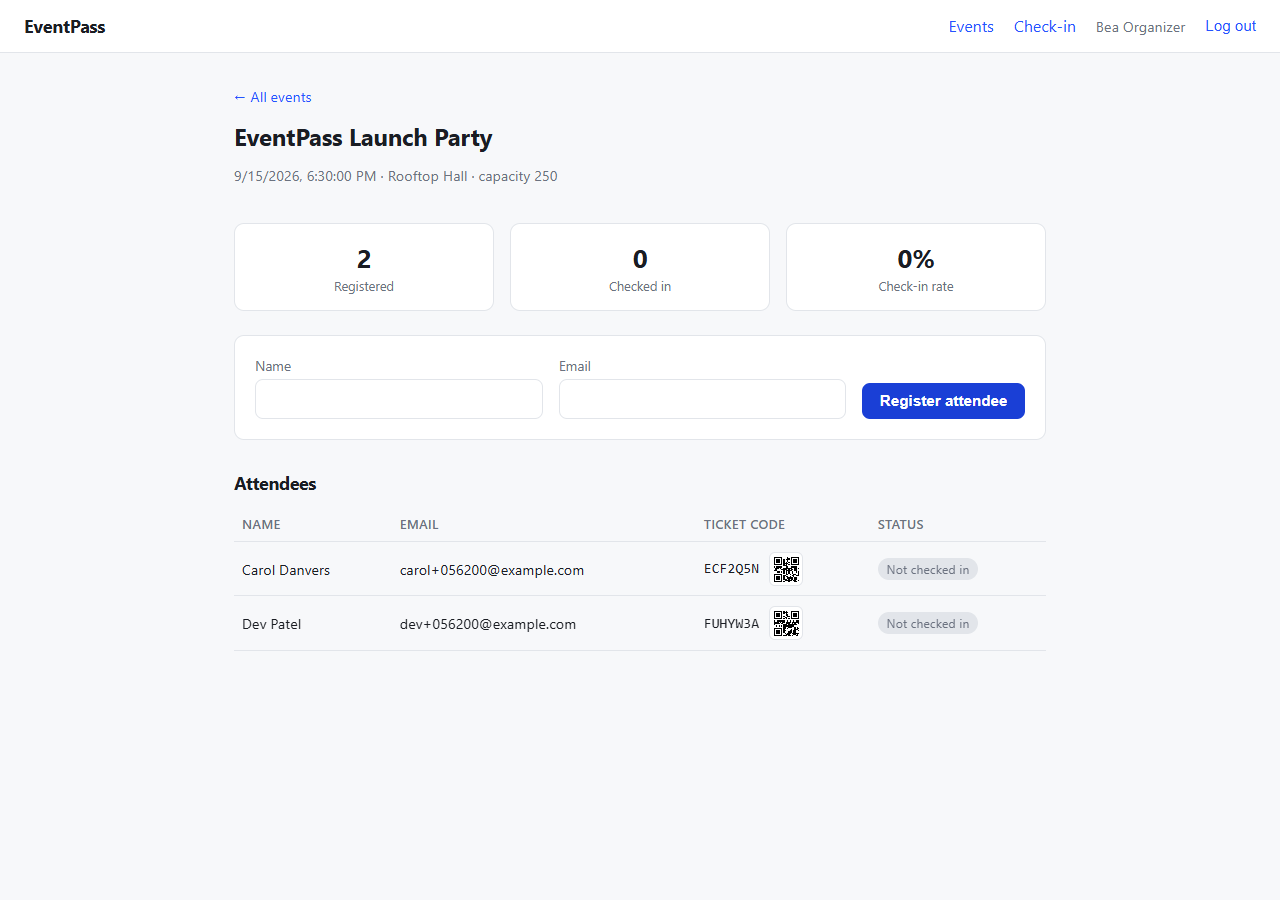
\includegraphics[width=0.85\textwidth]{04-attendees.png}
  \caption{Event detail page: attendee table with ticket codes and QR thumbnails.}
\end{figure}

\begin{figure}[h]
  \centering
  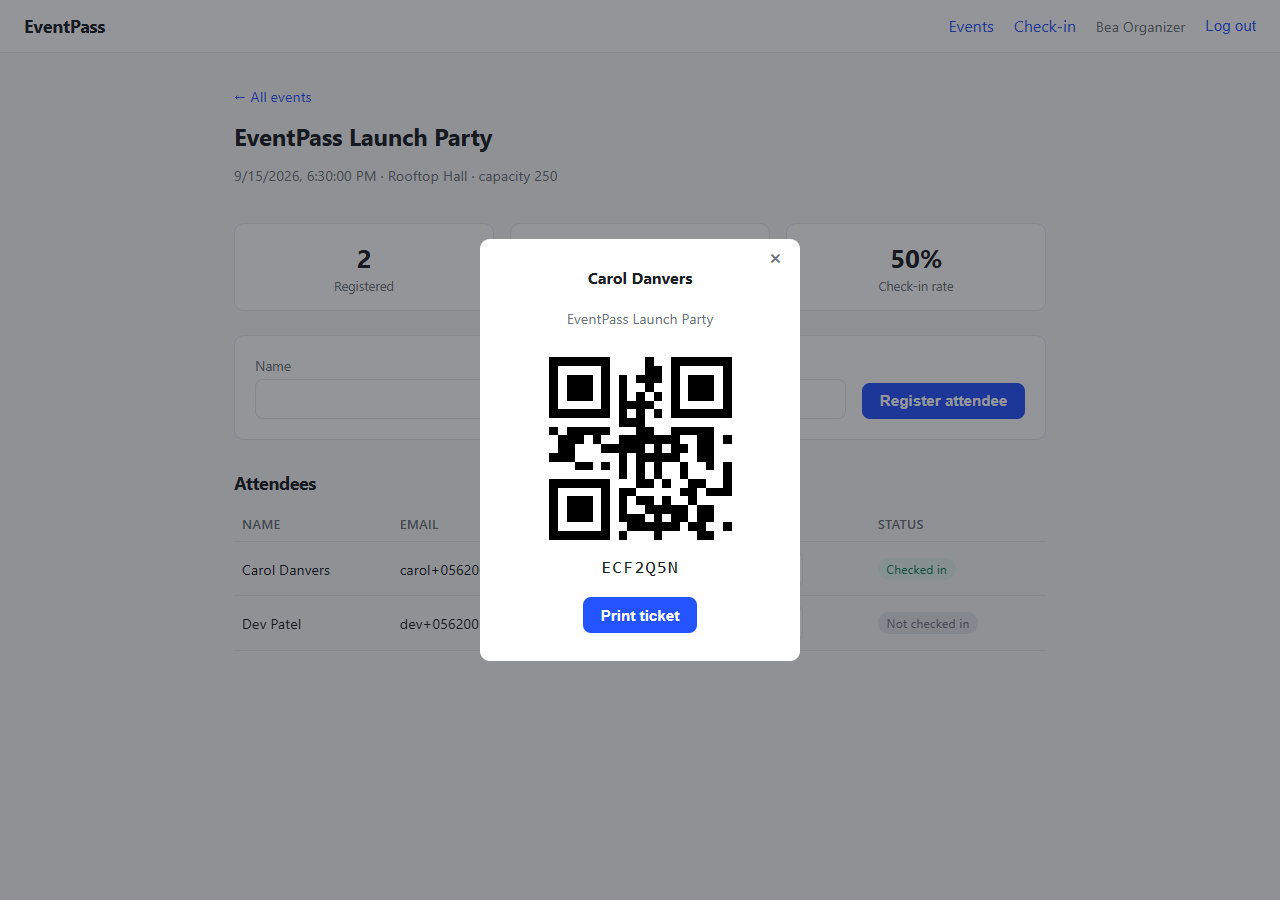
\includegraphics[width=0.7\textwidth]{10-qr-modal.png}
  \caption{Enlarged, printable QR ticket modal.}
\end{figure}

\begin{figure}[h]
  \centering
  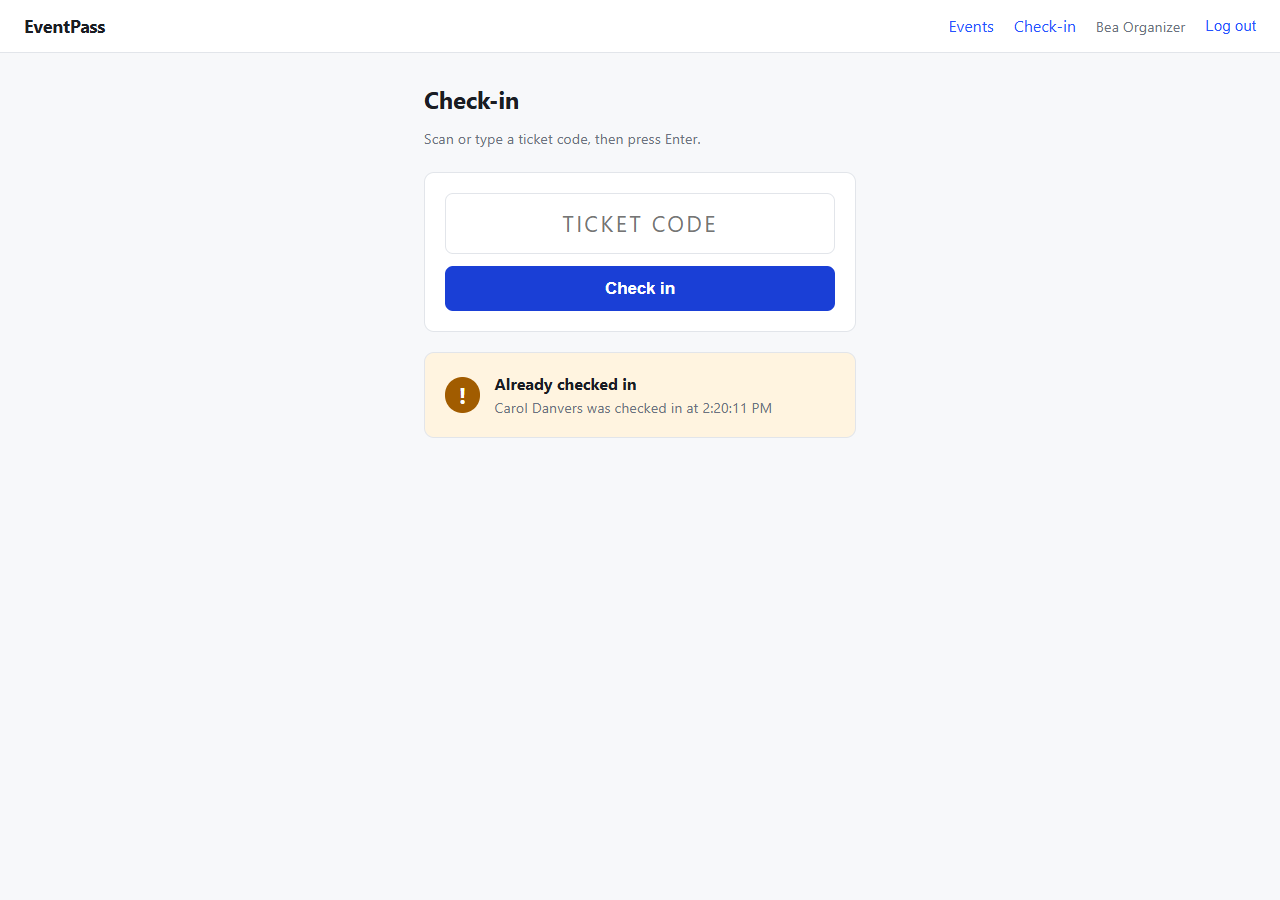
\includegraphics[width=0.6\textwidth]{07-checkin-duplicate.png}
  \caption{Check-in screen correctly refusing a duplicate scan.}
\end{figure}

\subsection{QR content verification}

Rendering a QR code is not proof it encodes the right value -- a
separate script decoded the rendered canvas pixel data with the
\code{jsQR} library and compared it against the ticket code shown in
the attendee table:

\begin{lstlisting}[caption={QR decode verification output}]
ticket code shown in table: PXDFR9Y
QR decoded value:           PXDFR9Y
MATCH: true
\end{lstlisting}

\subsection{A real bug found by this process}

Driving the UI in an actual browser (rather than only checking HTTP
status codes of the served files) surfaced a bug that request-level
checks could not: \code{frontend/src/auth.jsx} imported
\code{'../api/client'}, but since \code{auth.jsx} lives at
\code{src/auth.jsx} (not inside a subdirectory like the page
components that also use that import path), the relative path resolved
outside \code{src/} entirely. Vite failed the import and served an
error overlay -- with an HTTP \code{200} status, since Vite serves the
overlay as a successful response. The fix was a one-line change from
\code{'../api/client'} to \code{'./api/client'}. This is recorded here
because it is a useful illustration of why Chapter~\ref{ch:testing}'s
browser-driven verification exists at all: a purely HTTP-level smoke
test would have reported success on a completely broken frontend.

% ==================================================================
\chapter{Scope Boundaries}
\label{ch:scope}
% ==================================================================

The following were considered and deliberately left out, either
because the time-boxed build did not call for them or because they
would require product decisions outside this project's scope:

\begin{description}[leftmargin=2em, style=nextline]
  \item[Capacity enforcement] \code{events.capacity} is stored but
    nothing checks registered-attendee count against it -- an event
    can be over-registered with no warning.
  \item[Attendee-facing anything] No self-registration, no emailed
    ticket, no attendee login or ticket-status page. An organizer must
    deliver the ticket code/QR to the attendee out-of-band; the
    ``print ticket'' button exists for this purpose.
  \item[Undo check-in] Once checked in, there is no API to reverse it
    (e.g.\ for a mis-scan) short of editing the database directly.
  \item[Multi-organizer / per-event staff accounts] One organizer
    equals one login with full access to their own events. There is
    no way to grant a door-staff account restricted to check-in only.
  \item[Password reset, email verification, auth rate limiting]
    Registration and login are functional but bare -- no forgot-
    password flow, no lockout after repeated failed logins.
  \item[Payments / paid ticketing] ``Ticket'' here means an admission
    record, not a purchased good -- there is no price and no payment
    integration.
\end{description}

\end{document}
